%======================================================================
\section{Xu's switches and conditional timing}\label{app:xu}
Xu (2024) starts from the Moreira--Muir rule and adds two switches (his eq.~11),
\[
w_t=C_t\Bigl(\frac{c^*}{RV_{t-1}}\Bigr)^{I_t},
\]
where $c^*$ is a fixed target variance (12\% a year) and $I_t$, $C_t$ are two 0/1 switches set with data up to month $t-1$: an intercept switch ($I_t=0$, so $w_t=1$ and no timing, if the 60-month regression of returns on last month's variance has a non-positive intercept) and a cash switch ($C_t=0$, cash, if the past 12 months' return is negative). Conditional timing (Bongaerts et al., 2020) applies our rule only in the calmest and most volatile 20\% of months.

\begin{table}[htbp]
\centering\small
\caption{Xu's switches on top of our GARCH(1,1) rule, 1998--2025, net of costs.}\label{tab:xu}
\begin{adjustbox}{max width=\linewidth}\begin{tabular}{@{}lccccccc@{}}
\toprule
Rule & SR 98--25 & SR 98--15 & SR 16--25 & Sortino & Max DD eq.\ vol, \% & MT & VT\\
\midrule
Timed, GARCH(1,1) (ours) & 0.608 & 0.460 & 0.828 & 0.909 & $-$36.9 & 0.974 & 1.269\\
+ intercept switch only & 0.589 & 0.435 & 0.833 & 0.875 & $-$47.8 & 0.976 & 1.221\\
+ cash switch only & 0.657 & 0.589 & 0.765 & 1.005 & $-$28.4 & 1.096 & 1.218\\
+ both (Xu switches) & 0.679 & 0.625 & 0.771 & 1.045 & $-$28.7 & 1.141 & 1.203\\
Xu as in his paper & 0.615 & 0.622 & 0.615 & 0.924 & $-$34.4 & 1.100 & 1.147\\
Conditional (Bongaerts et al.) & 0.619 & 0.449 & 0.878 & 0.933 & $-$40.9 & 1.035 & 1.199\\
\bottomrule
\end{tabular}\end{adjustbox}
\end{table}

The cash switch, a time-series momentum filter (Moskowitz et al., 2012), does most of the work: it gains on the return side (MT 1.14), not through better volatility timing. Against buy and hold Xu's switches gain $+$0.16 of Sharpe (bootstrap $p=0.35$), $+$0.28 before 2016 and $-$0.05 after; not significant.

%======================================================================
\section{Building the rule one piece at a time}\label{app:buildup}

\begin{table}[htbp]
\centering\small
\caption{Rule build-up with the GARCH(1,1) forecast, 1998--2025; drawdowns and vol of vol at buy and hold's volatility.}\label{tab:buildup}
\begin{adjustbox}{max width=\linewidth}\begin{tabular}{@{}lcccccc@{}}
\toprule
Step & Sharpe & Sortino & Max DD, \% & Vol of vol, \% & Traded/yr & MT\\
\midrule
1. Buy and hold & 0.516 & 0.748 & $-$50.3 & 5.76 & 0.00 & 1.000\\
2. Scale by $1/\sigma$ (vol target), no cap, no costs & 0.614 & 0.908 & $-$42.8 & 3.51 & 2.36 & 0.986\\
3. Scale by $1/\sigma^2$ instead (Moreira--Muir) & 0.608 & 0.897 & $-$34.1 & 5.17 & 3.89 & 0.953\\
4. + cap exposure at 1.5 & 0.637 & 0.960 & $-$36.4 & 4.20 & 3.28 & 0.974\\
5. + 10 bp trading costs (our rule) & 0.608 & 0.909 & $-$36.9 & 4.19 & 3.28 & 0.974\\
6. $c$ set once (1970--1997) instead of every January & 0.574 & 0.843 & $-$39.3 & 4.17 & 3.24 & 0.932\\
\bottomrule
\end{tabular}\end{adjustbox}
\end{table}

Volatility scaling (Harvey et al., 2018) already lifts the Sharpe ratio to 0.61; variance scaling cuts the drawdown more but lowers MT; the cap helps a little; costs take 0.03; a frozen $c$ loses 0.03 more. Moreira and Muir's full-sample $c$, which looks ahead, gives a lower Sharpe ratio than our real-time $c$ for all five forecasts (by 0.02 to 0.03).

%======================================================================
\section{The six factors and factor exposure over time}\label{app:factors}
Timed on its own GARCH(1,1) forecast, the average Sharpe gain across the six factors is about zero ($+$0.01; 2 of 6 gain), with a smaller drawdown on 4 of 6. Momentum has the largest gain ($+$0.35, Ledoit--Wolf $p=0.02$, Romano--Wolf $p=0.10$), in line with Barroso and Santa-Clara (2015). Figure~\ref{fig:factorexp} shows that the models cut every factor together in crises. The accuracy-trained GJR-GARCH and GARCH-LSTM hold almost the same exposures; only the decision-trained network departs, holding more of the market, SMB and RMW (average SMB exposure 0.83 against 0.77) and less of momentum and CMA.

\begin{figure}[htbp]
\centering
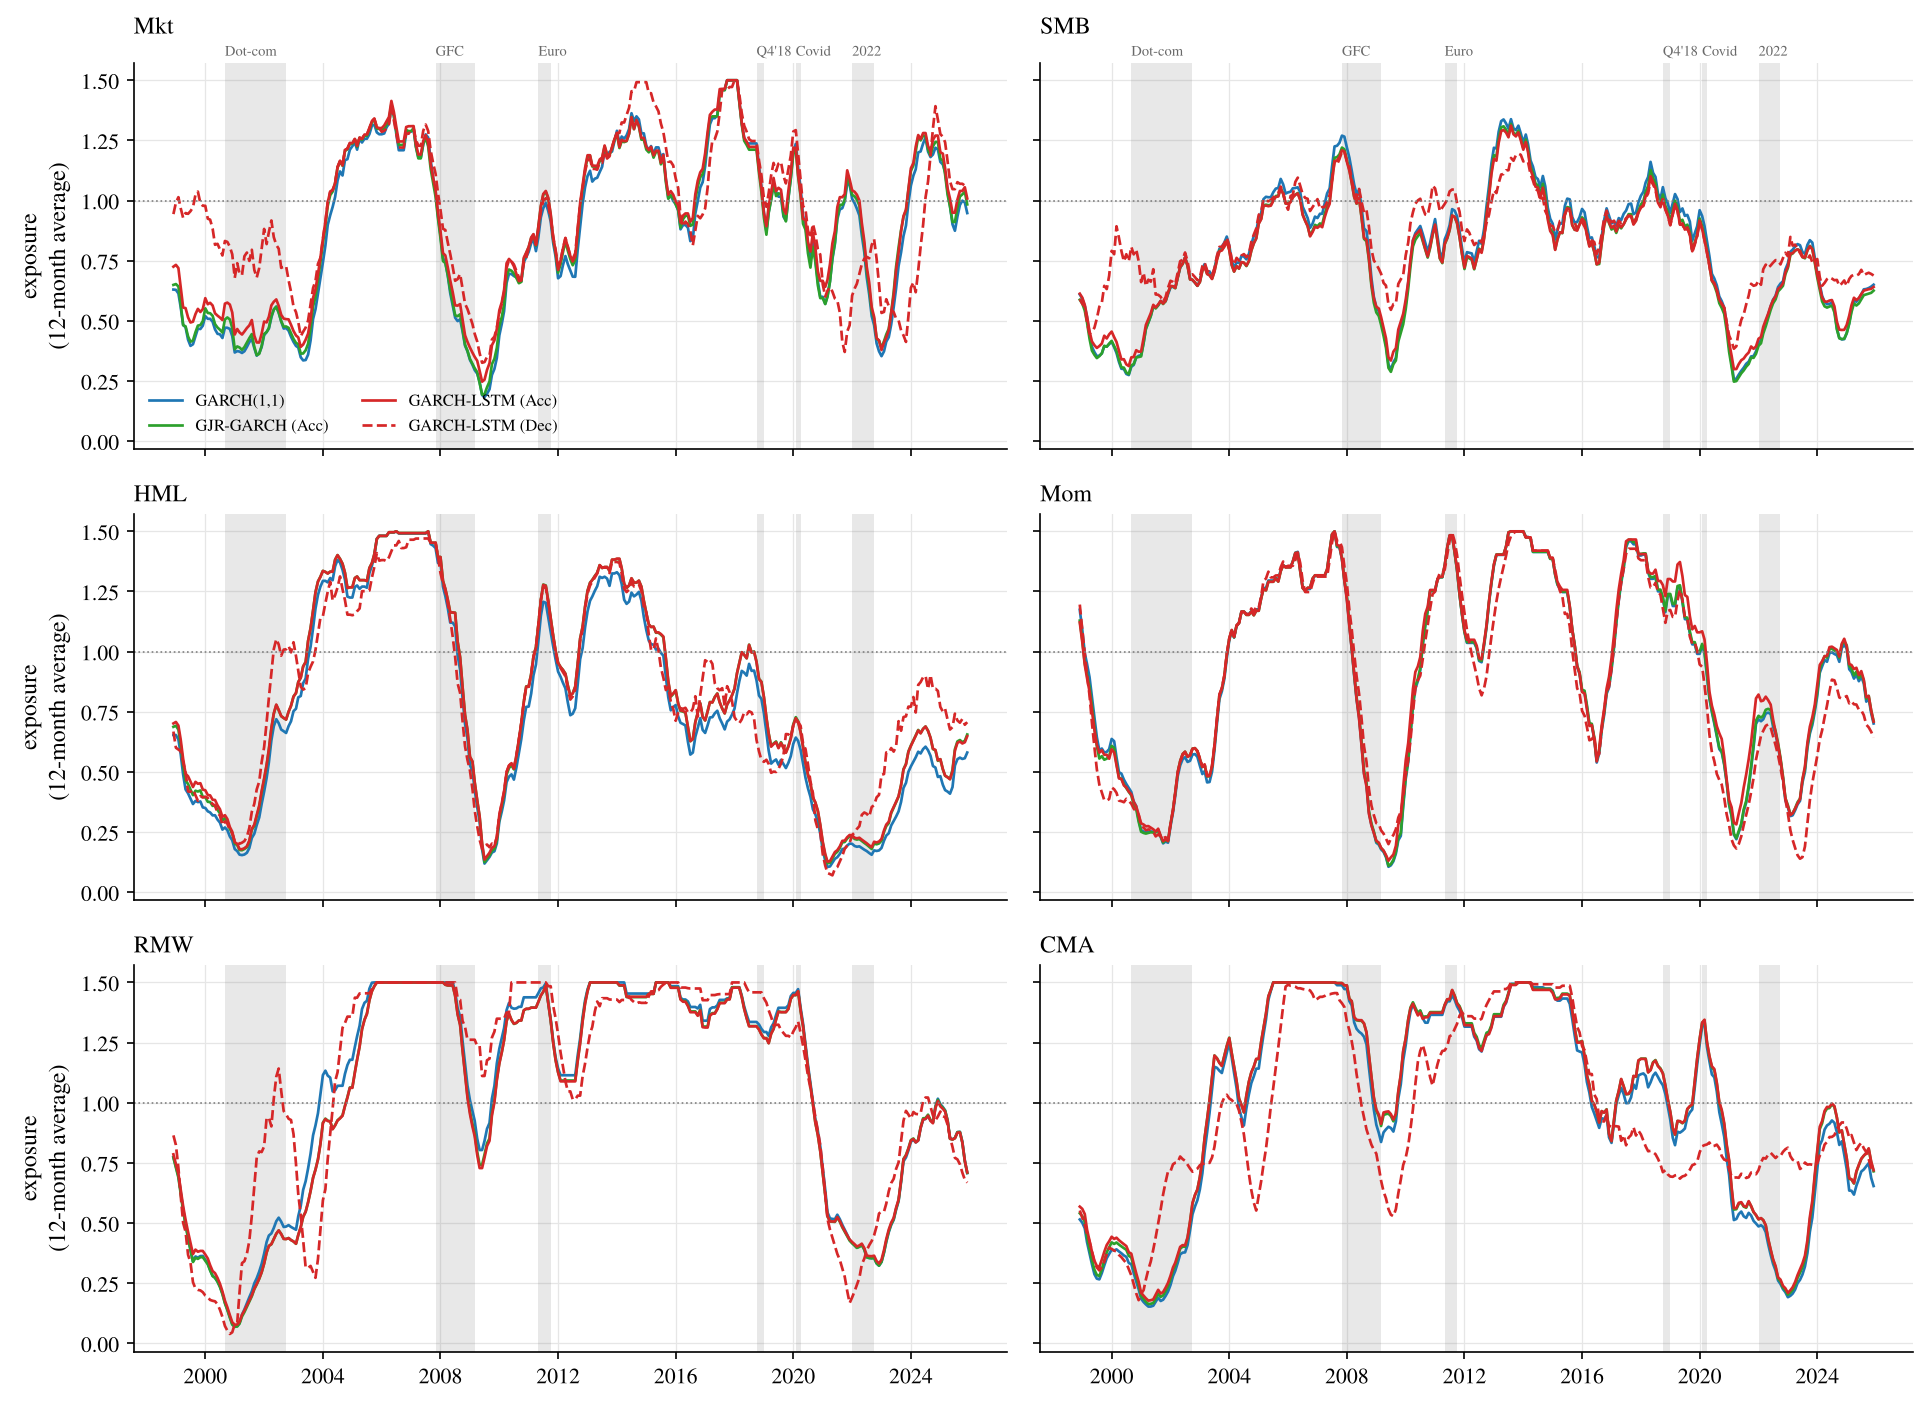
\includegraphics[width=\textwidth]{figs/figC_factor_exposures.png}
\caption{Exposure to each factor (12-month average) under each forecast, 1998--2025. Grey bands: the six crises.}
\label{fig:factorexp}
\end{figure}

%======================================================================
\section{Further checks}\label{app:checks}
\begin{figure}[htbp]
\centering
\begin{subfigure}[t]{0.42\textwidth}\centering
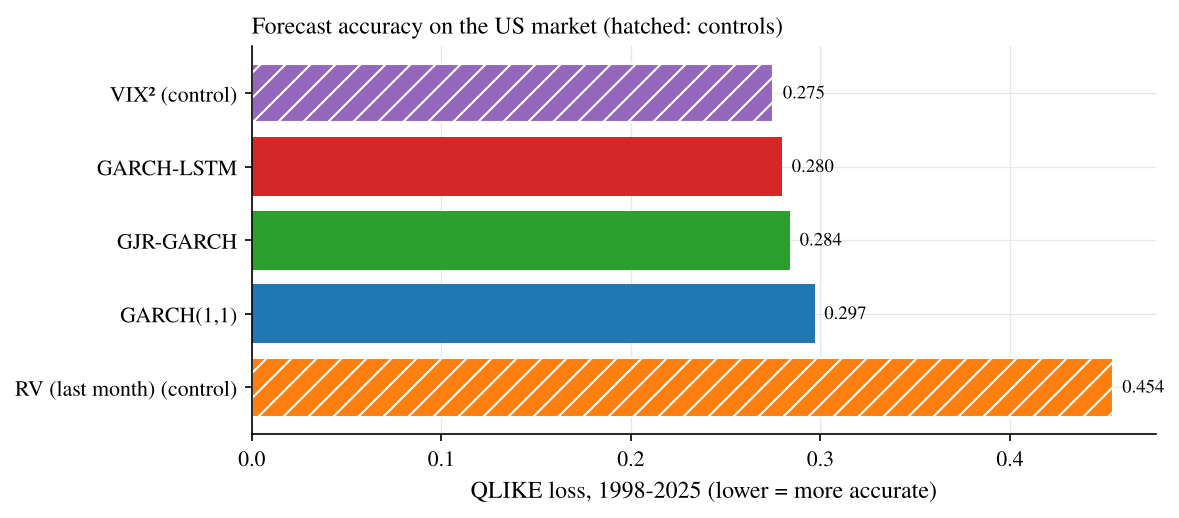
\includegraphics[width=\textwidth]{figs/fig04_qlike.png}
\caption{QLIKE, 1998--2025.}
\end{subfigure}\hfill
\begin{subfigure}[t]{0.55\textwidth}\centering
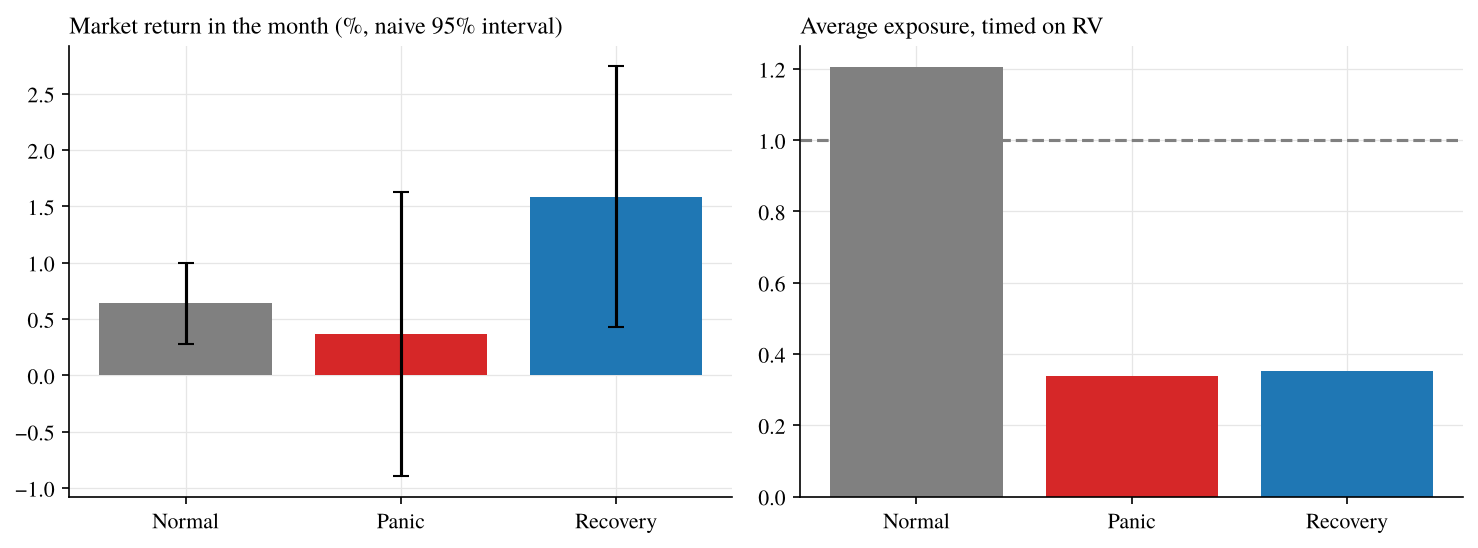
\includegraphics[width=\textwidth]{figs/fig05_recovery.png}
\caption{Recovery months, 1975--2025.}
\end{subfigure}
\caption{Forecast accuracy and the recovery months.}
\label{fig:qlike}
\end{figure}

\begin{figure}[htbp]
\centering
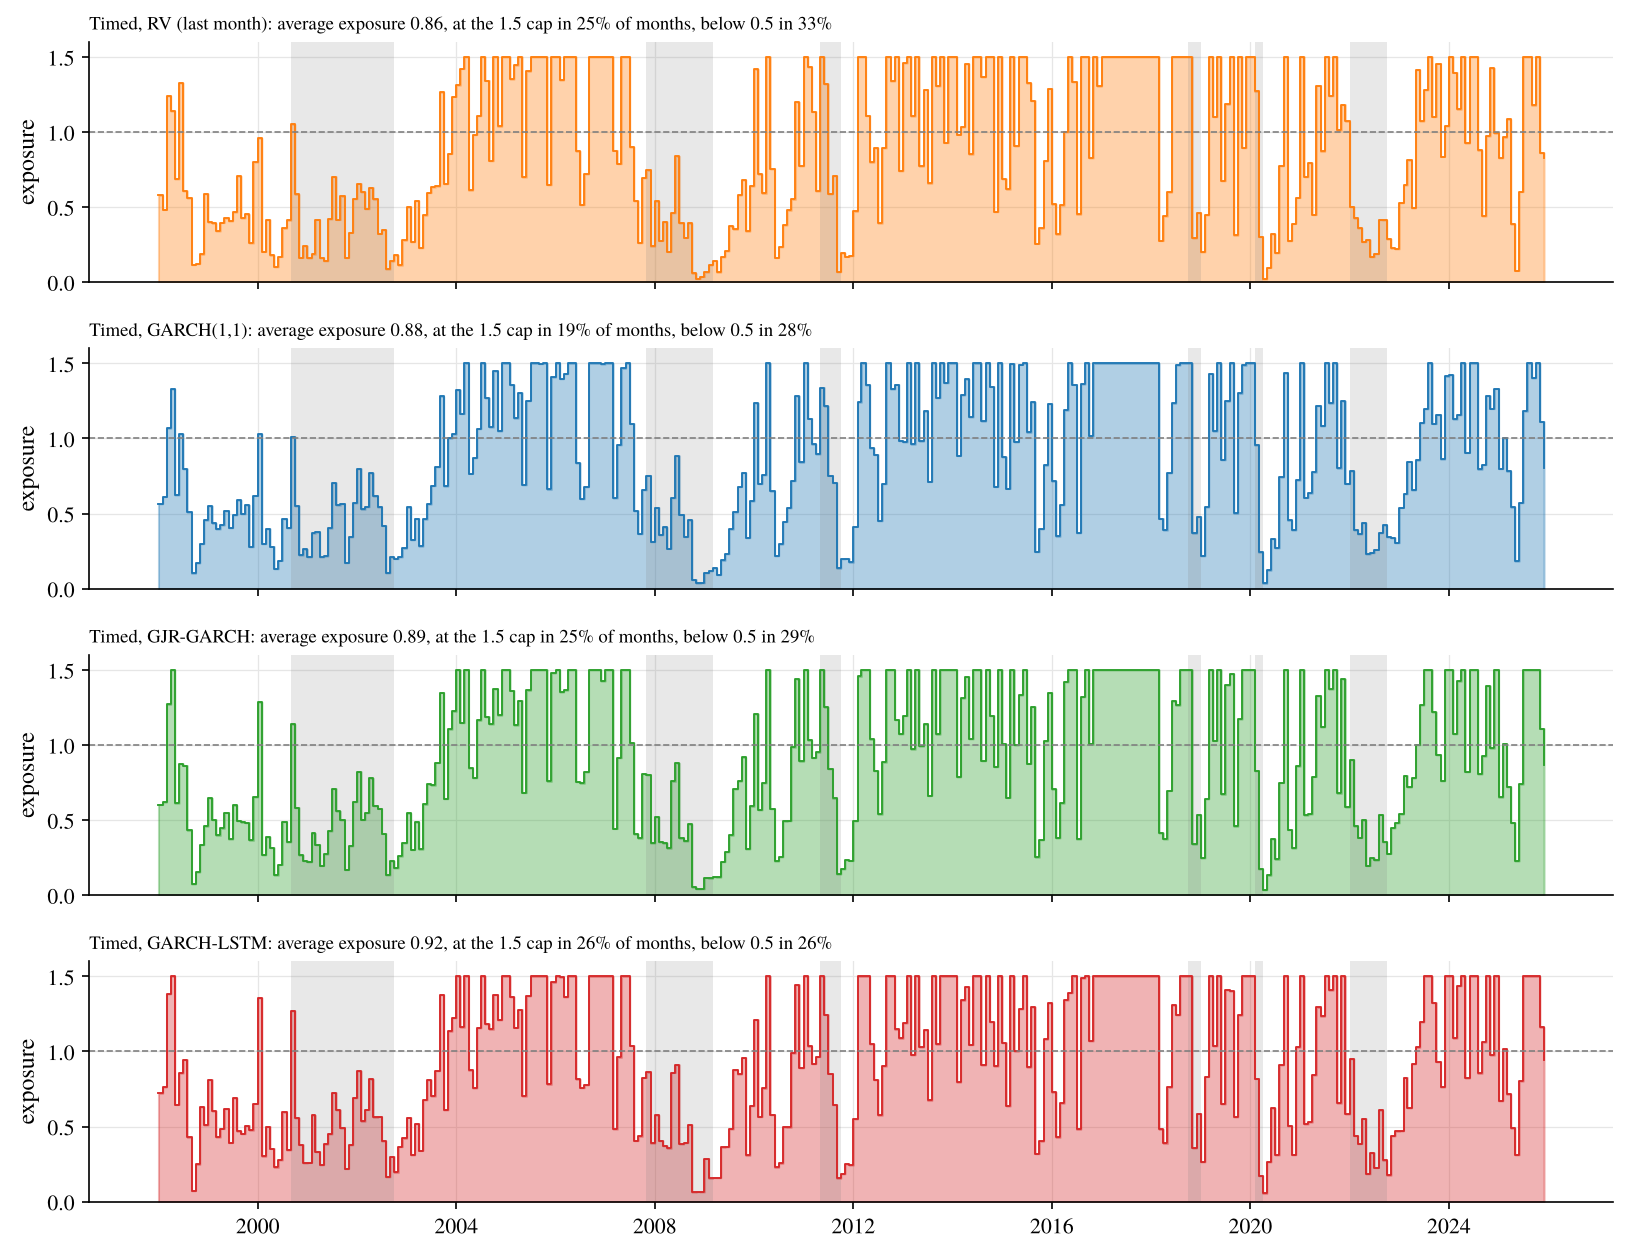
\includegraphics[width=0.72\textwidth]{figs/figE_exposures.png}
\caption{Monthly market exposure chosen by the rule for each timed model, 1998--2025.}
\label{fig:exposures}
\end{figure}

\paragraph{QLIKE by sub-period.} GJR-GARCH and the GARCH-LSTM are the most accurate forecasts in 1998--2015 (both 0.235), \VIX{} in 2016--2025 (0.314, against 0.360 for the GARCH-LSTM) and the GARCH-LSTM in 2021--2025 (0.178); RV is the least accurate everywhere. The Ledoit--Wolf $p$-values of the main comparisons barely move with 0 to 12 HAC lags (e.g.\ GARCH(1,1) vs buy and hold: 0.44 to 0.48).

\paragraph{Reproducibility.} All results come from \texttt{vol\_timing\_final\_revised.ipynb}. The GJR-GARCH and GARCH-LSTM forecasts, scales and exposures come from the full run of \texttt{lstm\_training\_revised.ipynb} (six factors, five seeds, test years 1975--2025), saved in \texttt{data/LSTM-Forecasts-revised/}. The figures in this report were regenerated by running the notebook; the portfolio value curves, calendar-year returns, rolling Sharpe ratios and the extended performance table (CAGR, Calmar ratio, CAPM alpha and beta) are computed from the notebook's own backtest series by \texttt{report\_extras.py}, and the robustness checks quoted in the separate responses to questions by \texttt{qa\_checks.py}. The licensed course CRSP file is not redistributed; without it, only the CRSP benchmark is skipped.
